\documentclass[12pt,a4paper]{article}
\usepackage[a4paper,margin=1in]{geometry}
\usepackage{amsmath,amssymb,graphicx,float,booktabs}
\usepackage{xcolor}
\usepackage{microtype}
\usepackage[hidelinks]{hyperref}

\definecolor{accent}{HTML}{174A5B}
\definecolor{lightaccent}{HTML}{EAF3F5}
\hypersetup{colorlinks=true,linkcolor=accent,urlcolor=accent}

\title{\textbf{INCM Assignment 2}\\[4pt]\large Hodgkin--Huxley Dynamics and a Cav3.1 Calcium Channel}
\author{Nisarg Suthar \quad -- \quad 2026900002}
\date{}

\begin{document}
\maketitle

\begin{center}
\colorbox{lightaccent}{\parbox{0.92\textwidth}{\small
This report summarizes the simulations in the accompanying Python notebook. The
models use the classical Hodgkin--Huxley voltage convention, in which the resting
potential is approximately $0\,\mathrm{mV}$, and the Cav3.1 equations are converted
from Channelpedia voltage coordinates as described below.}}
\end{center}

\section*{Overview}
The assignment examines action-potential generation in the classical Hodgkin--Huxley
(HH) model, measures how sodium conductance changes repetitive firing, and extends the
model with a low-threshold Cav3.1 calcium channel to test rebound firing after
hyperpolarization. Simulations use Brian2 and the \texttt{exponential\_euler} method.

\section*{Part A: Classical Hodgkin--Huxley Model}
\subsection*{Q1: Dynamics of an action potential}
The HH membrane equation implemented by the model is
\begin{equation}
 C_m\frac{dV}{dt}=I_{\mathrm{ext}}+
 \bar g_{\mathrm{Na}}m^3h(E_{\mathrm{Na}}-V)+
 \bar g_{\mathrm{K}}n^4(E_{\mathrm{K}}-V)+g_{\mathrm{L}}(E_{\mathrm{L}}-V).
\end{equation}
Here $m$ is sodium activation, $h$ is sodium inactivation, and $n$ is potassium
activation. The notebook applies a $7.2\,\mu\mathrm{A}$ step from $10$ to $12\,\mathrm{ms}$,
simulates for $50\,\mathrm{ms}$, and uses $\Delta t=0.01\,\mathrm{ms}$.

\begin{figure}[H]
\centering
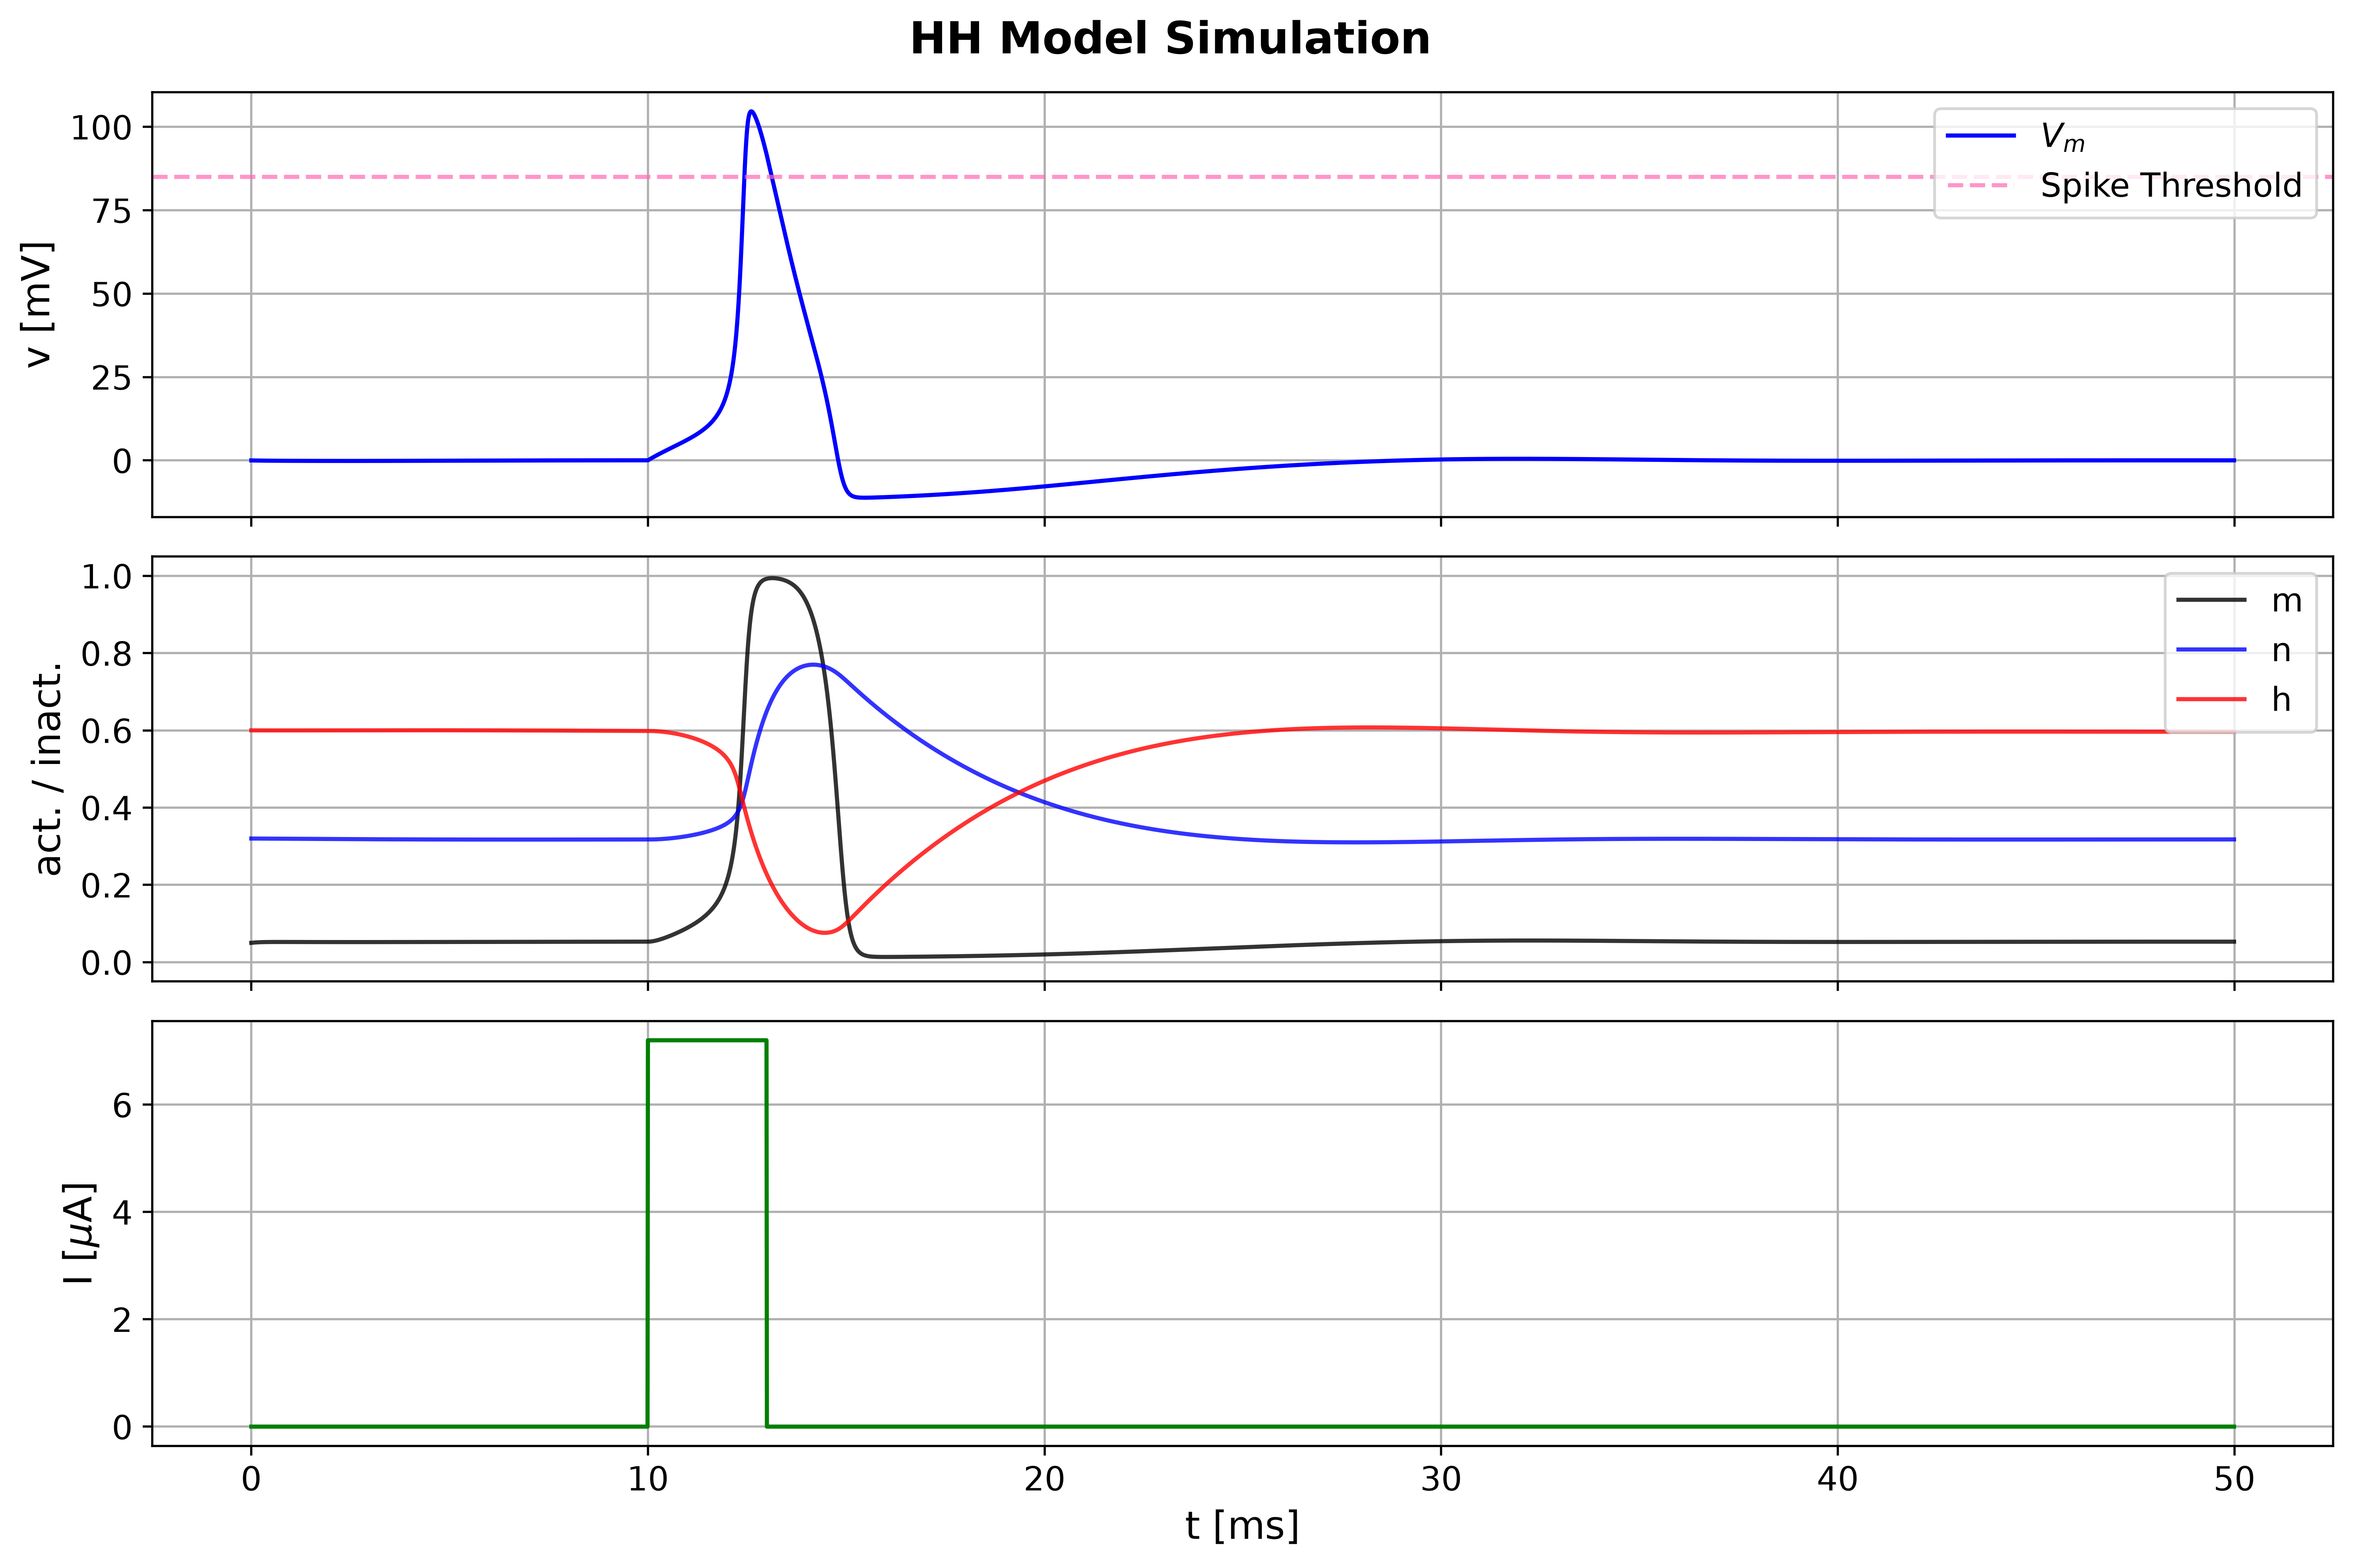
\includegraphics[width=0.94\textwidth]{../figures/q1/HH_sim.png}
\caption{Classical HH response to a brief depolarizing current step.}
\label{fig:q1}
\end{figure}

The neuron begins near the classical HH resting state, $V\approx0\,\mathrm{mV}$,
with $m\approx0.05$, $h\approx0.60$, and $n\approx0.32$. The current step rapidly
increases sodium activation. The resulting inward sodium current reinforces
 depolarization and produces the upstroke. Sodium inactivation and delayed potassium
activation then terminate the spike and produce the afterhyperpolarization. Recovery of
the gates returns the membrane toward rest.

\subsection*{Q2: Effect of sodium conductance on excitability}
 The standard model uses $\bar g_{\mathrm{Na}}=120\,\mathrm{mS}$; the modified model
uses $1.4\times120=168\,\mathrm{mS}$. A current step is applied from $50$ to
$350\,\mathrm{ms}$ during a $400\,\mathrm{ms}$ simulation. Currents are swept from
$0$ to $15\,\mu\mathrm{A}$ in increments of $0.1\,\mu\mathrm{A}$. Repetitive firing
means at least three upward crossings of $20\,\mathrm{mV}$ during the injection
interval. The threshold search uses $\Delta t=0.05\,\mathrm{ms}$.
The near-threshold traces are then generated at both $\Delta t=0.05\,\mathrm{ms}$
and the finer $\Delta t=0.01\,\mathrm{ms}$ to check that the qualitative comparison
is not an integration-step artifact.

\begin{table}[H]
\centering
\caption{Repetitive-firing thresholds obtained by the notebook search.}
\label{tab:thresholds}
\begin{tabular}{lccc}
\toprule
Model & $\bar g_{\mathrm{Na}}$ & $I_{\mathrm{th}}$ & Spikes at threshold\\
\midrule
Standard HH & $120\,\mathrm{mS}$ & $6.2\,\mu\mathrm{A}$ & 3\\
Modified HH & $168\,\mathrm{mS}$ & $1.2\,\mu\mathrm{A}$ & 13\\
\bottomrule
\end{tabular}
\end{table}

The measured threshold reduction is
\begin{equation}
\frac{6.2-1.2}{6.2}\times100\%\approx80.6\%.
\end{equation}
Increasing $\bar g_{\mathrm{Na}}$ strengthens the regenerative sodium feedback, so
less external current is needed to overcome leak and potassium currents. The modified
model also produces more spikes during the fixed $300\,\mathrm{ms}$ step, although
this count is a finite-window measure rather than an asymptotic firing rate.

\begin{figure}[H]
\centering
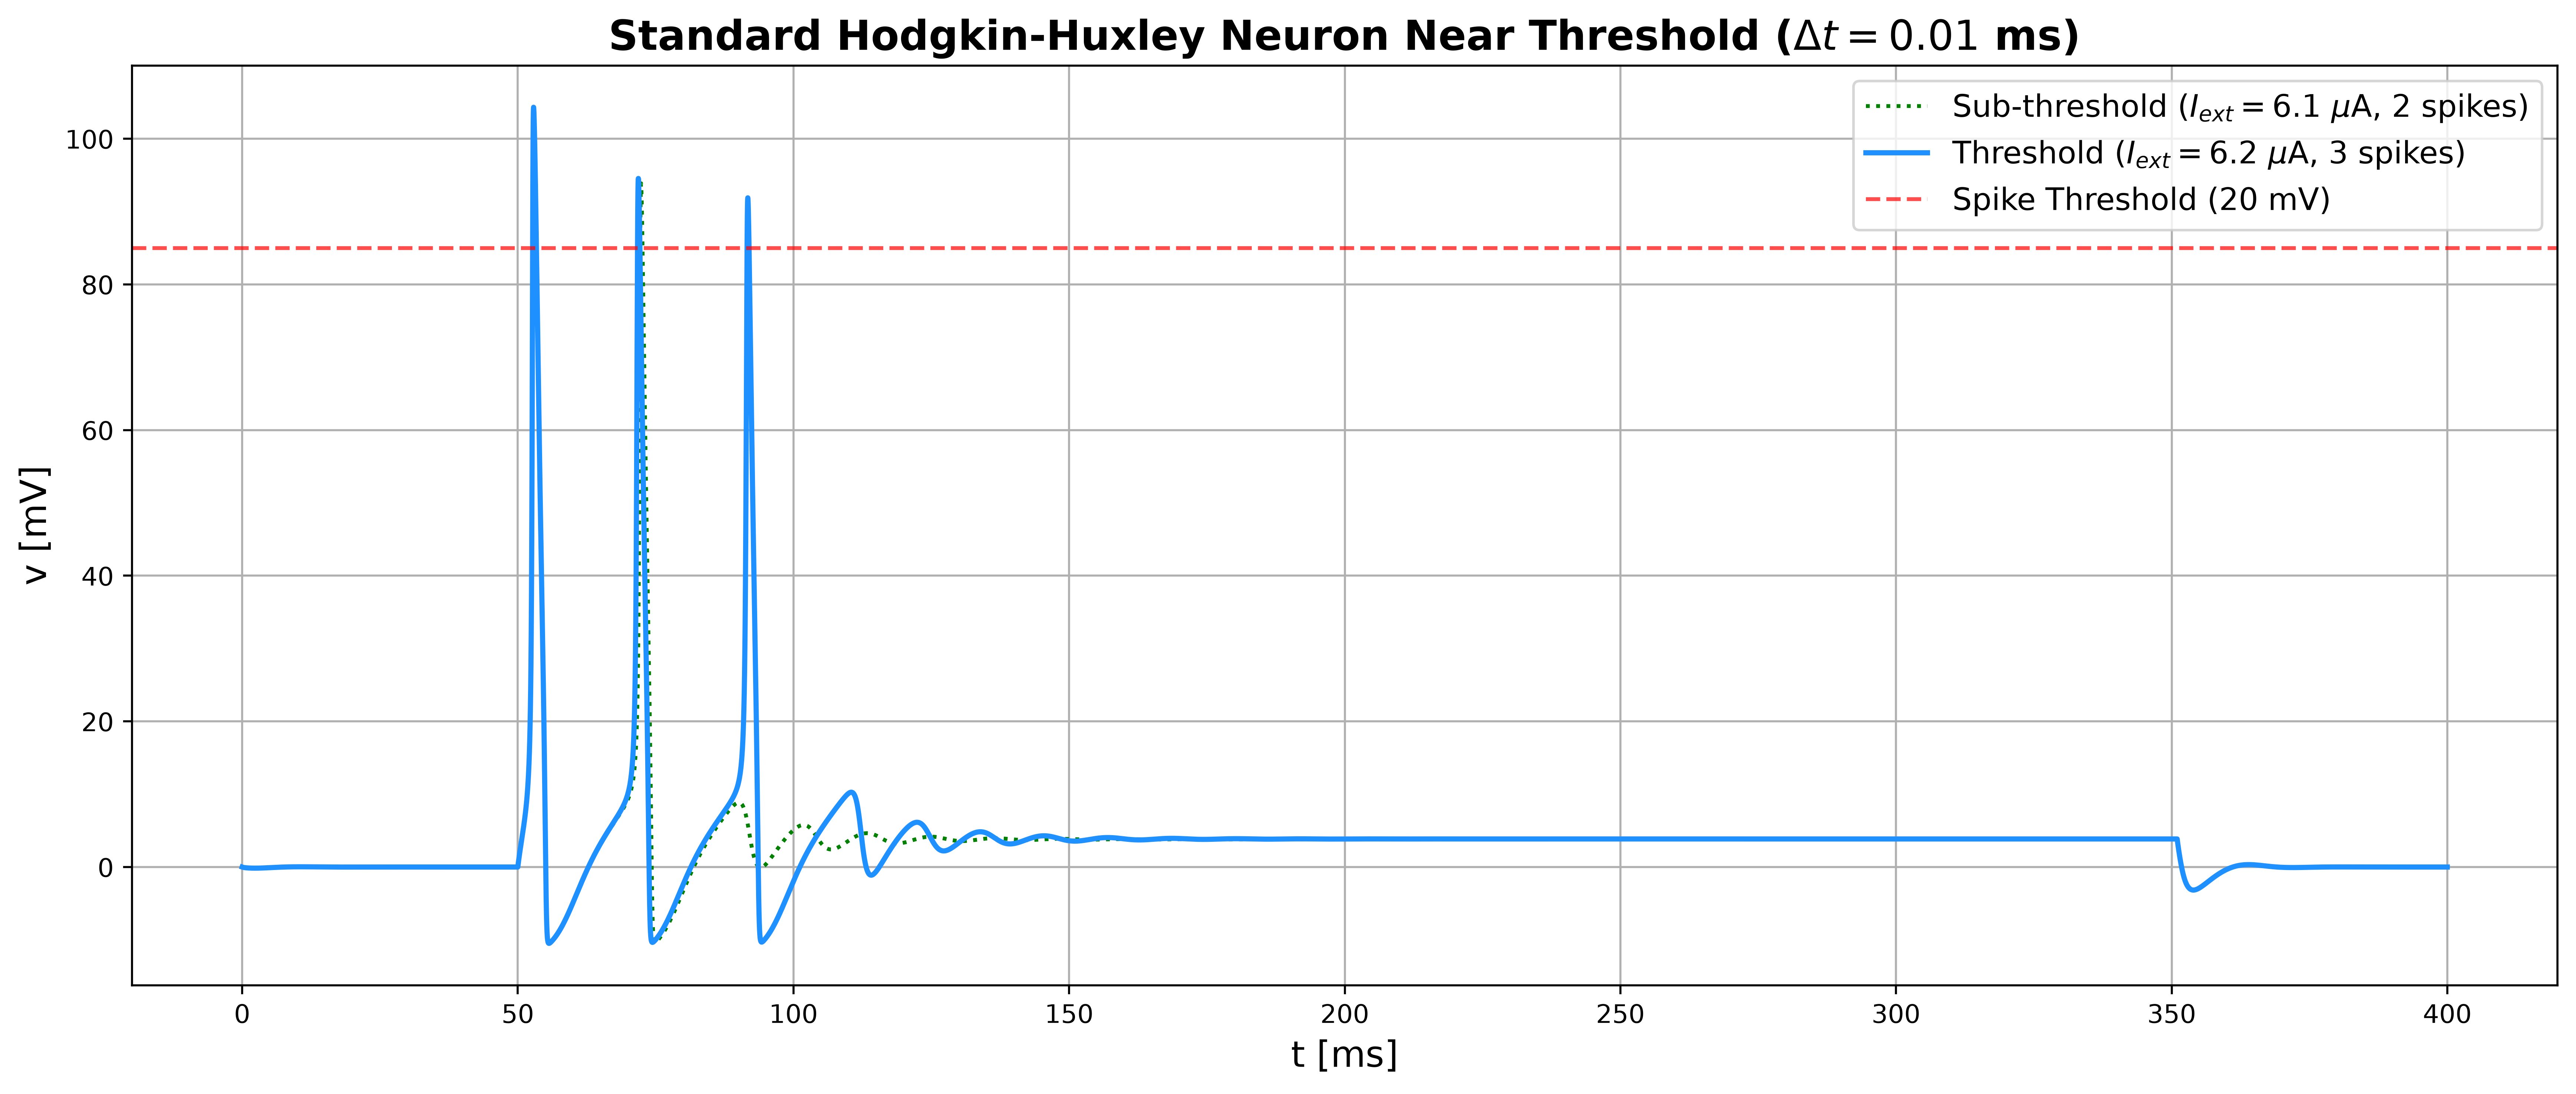
\includegraphics[width=0.94\textwidth]{../figures/q2/standard_hh_threshold_0.01.png}
\caption{Standard HH: a current just below the measured repetitive-firing threshold ($6.1\,\mu\mathrm{A}$, two spikes) compared with the threshold current ($6.2\,\mu\mathrm{A}$, three spikes), using $\Delta t=0.01\,\mathrm{ms}$.}
\label{fig:q2standard01}
\end{figure}
\begin{figure}[H]
\centering
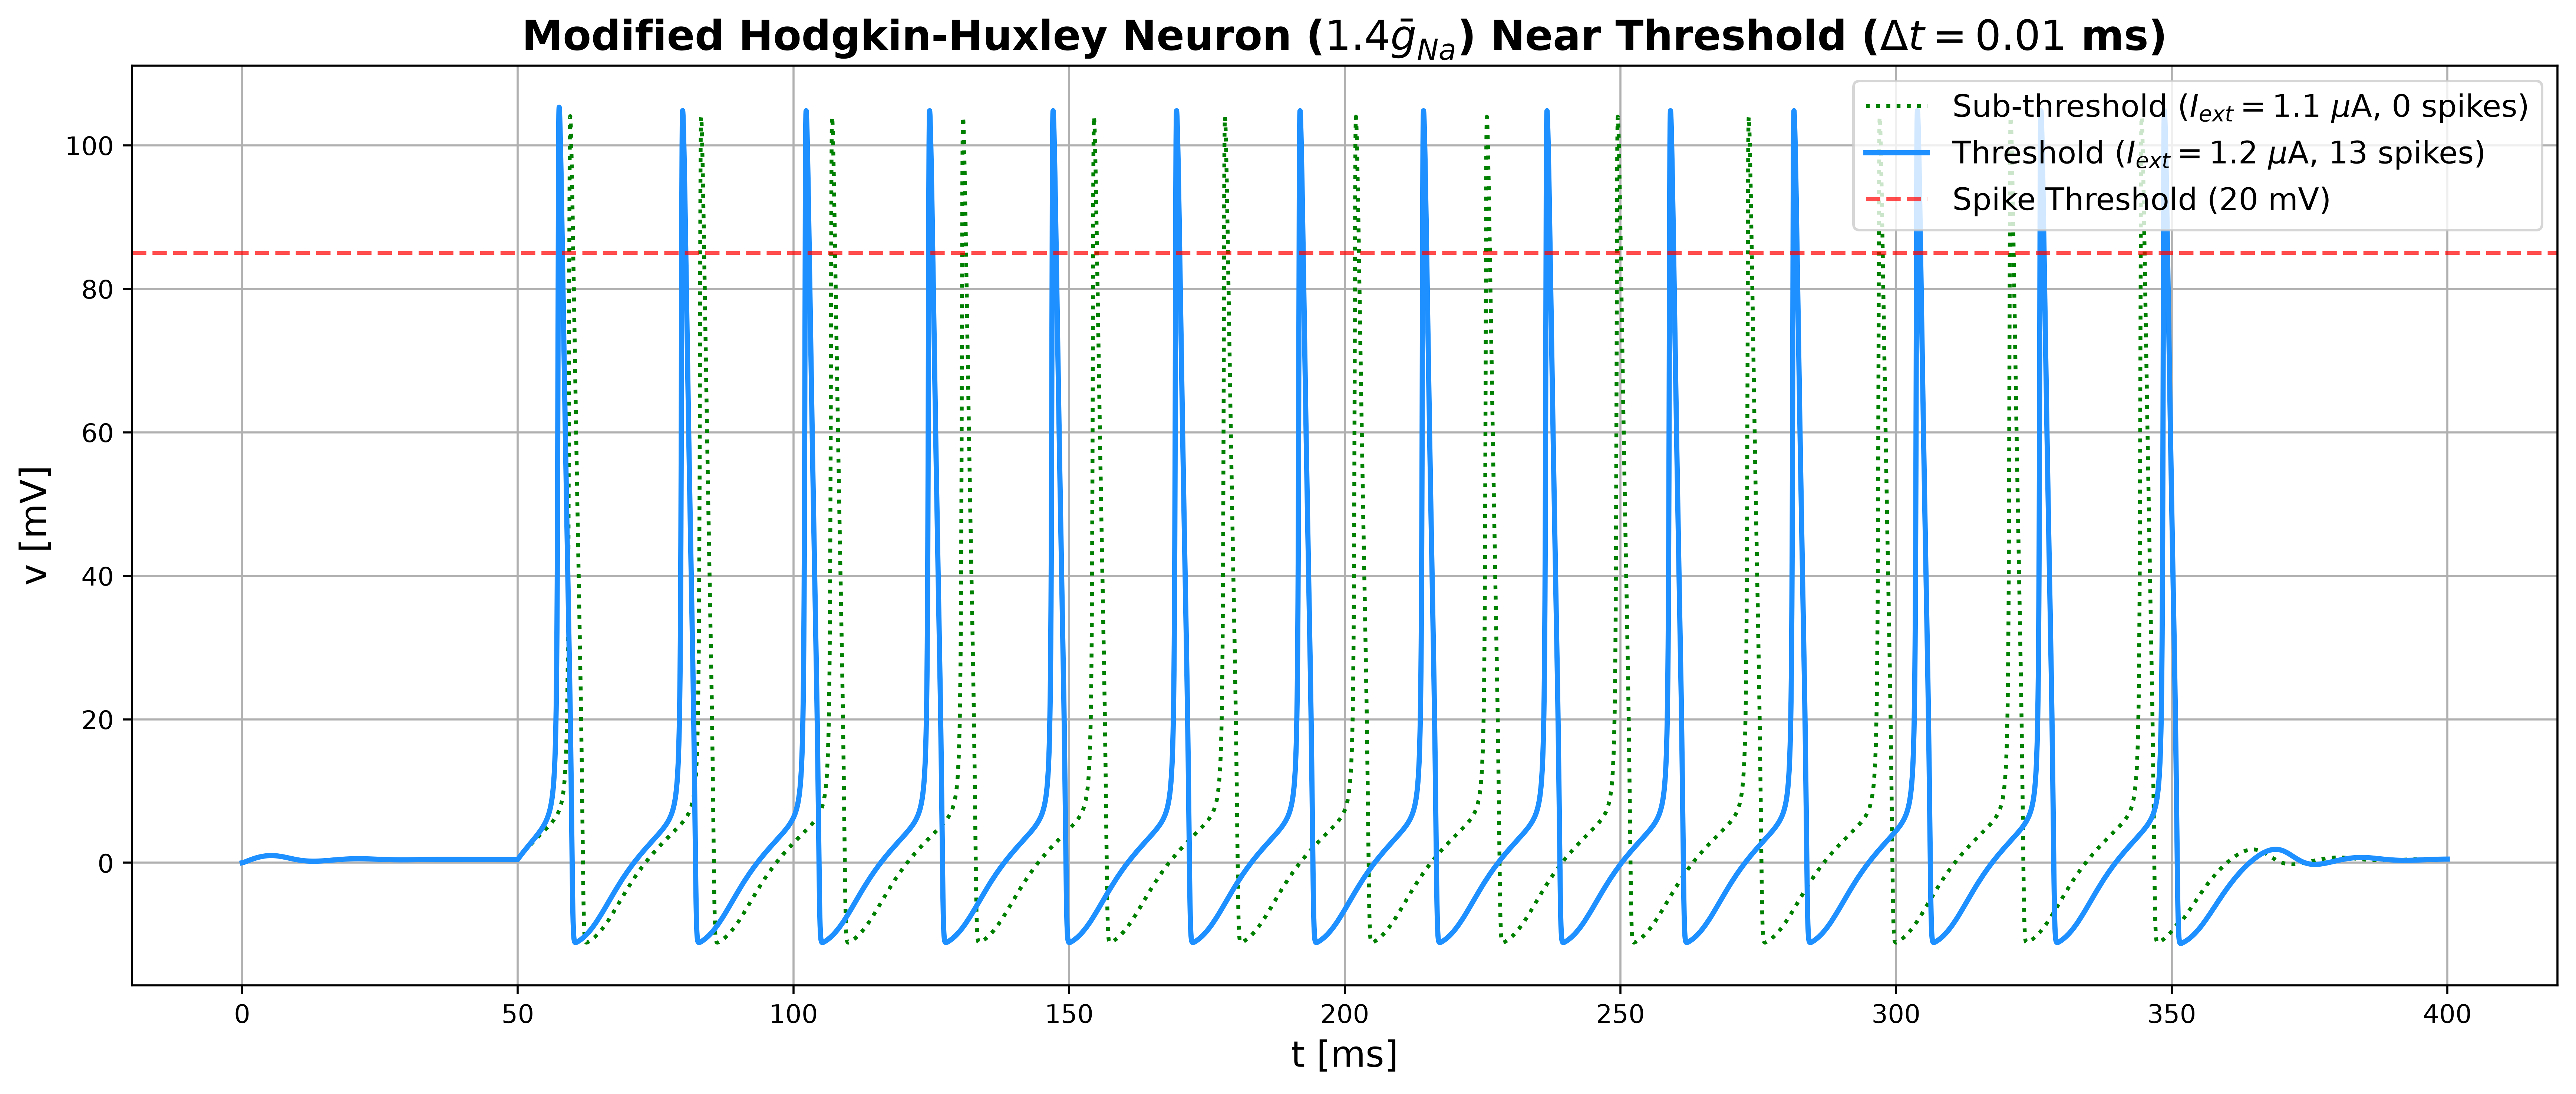
\includegraphics[width=0.94\textwidth]{../figures/q2/modified_hh_threshold_0.01.png}
\caption{Modified HH: a current below the measured repetitive-firing threshold ($1.1\,\mu\mathrm{A}$, no spikes) compared with the threshold current ($1.2\,\mu\mathrm{A}$, thirteen spikes), using $\Delta t=0.01\,\mathrm{ms}$.}
\label{fig:q2modified01}
\end{figure}
\begin{figure}[H]
\centering
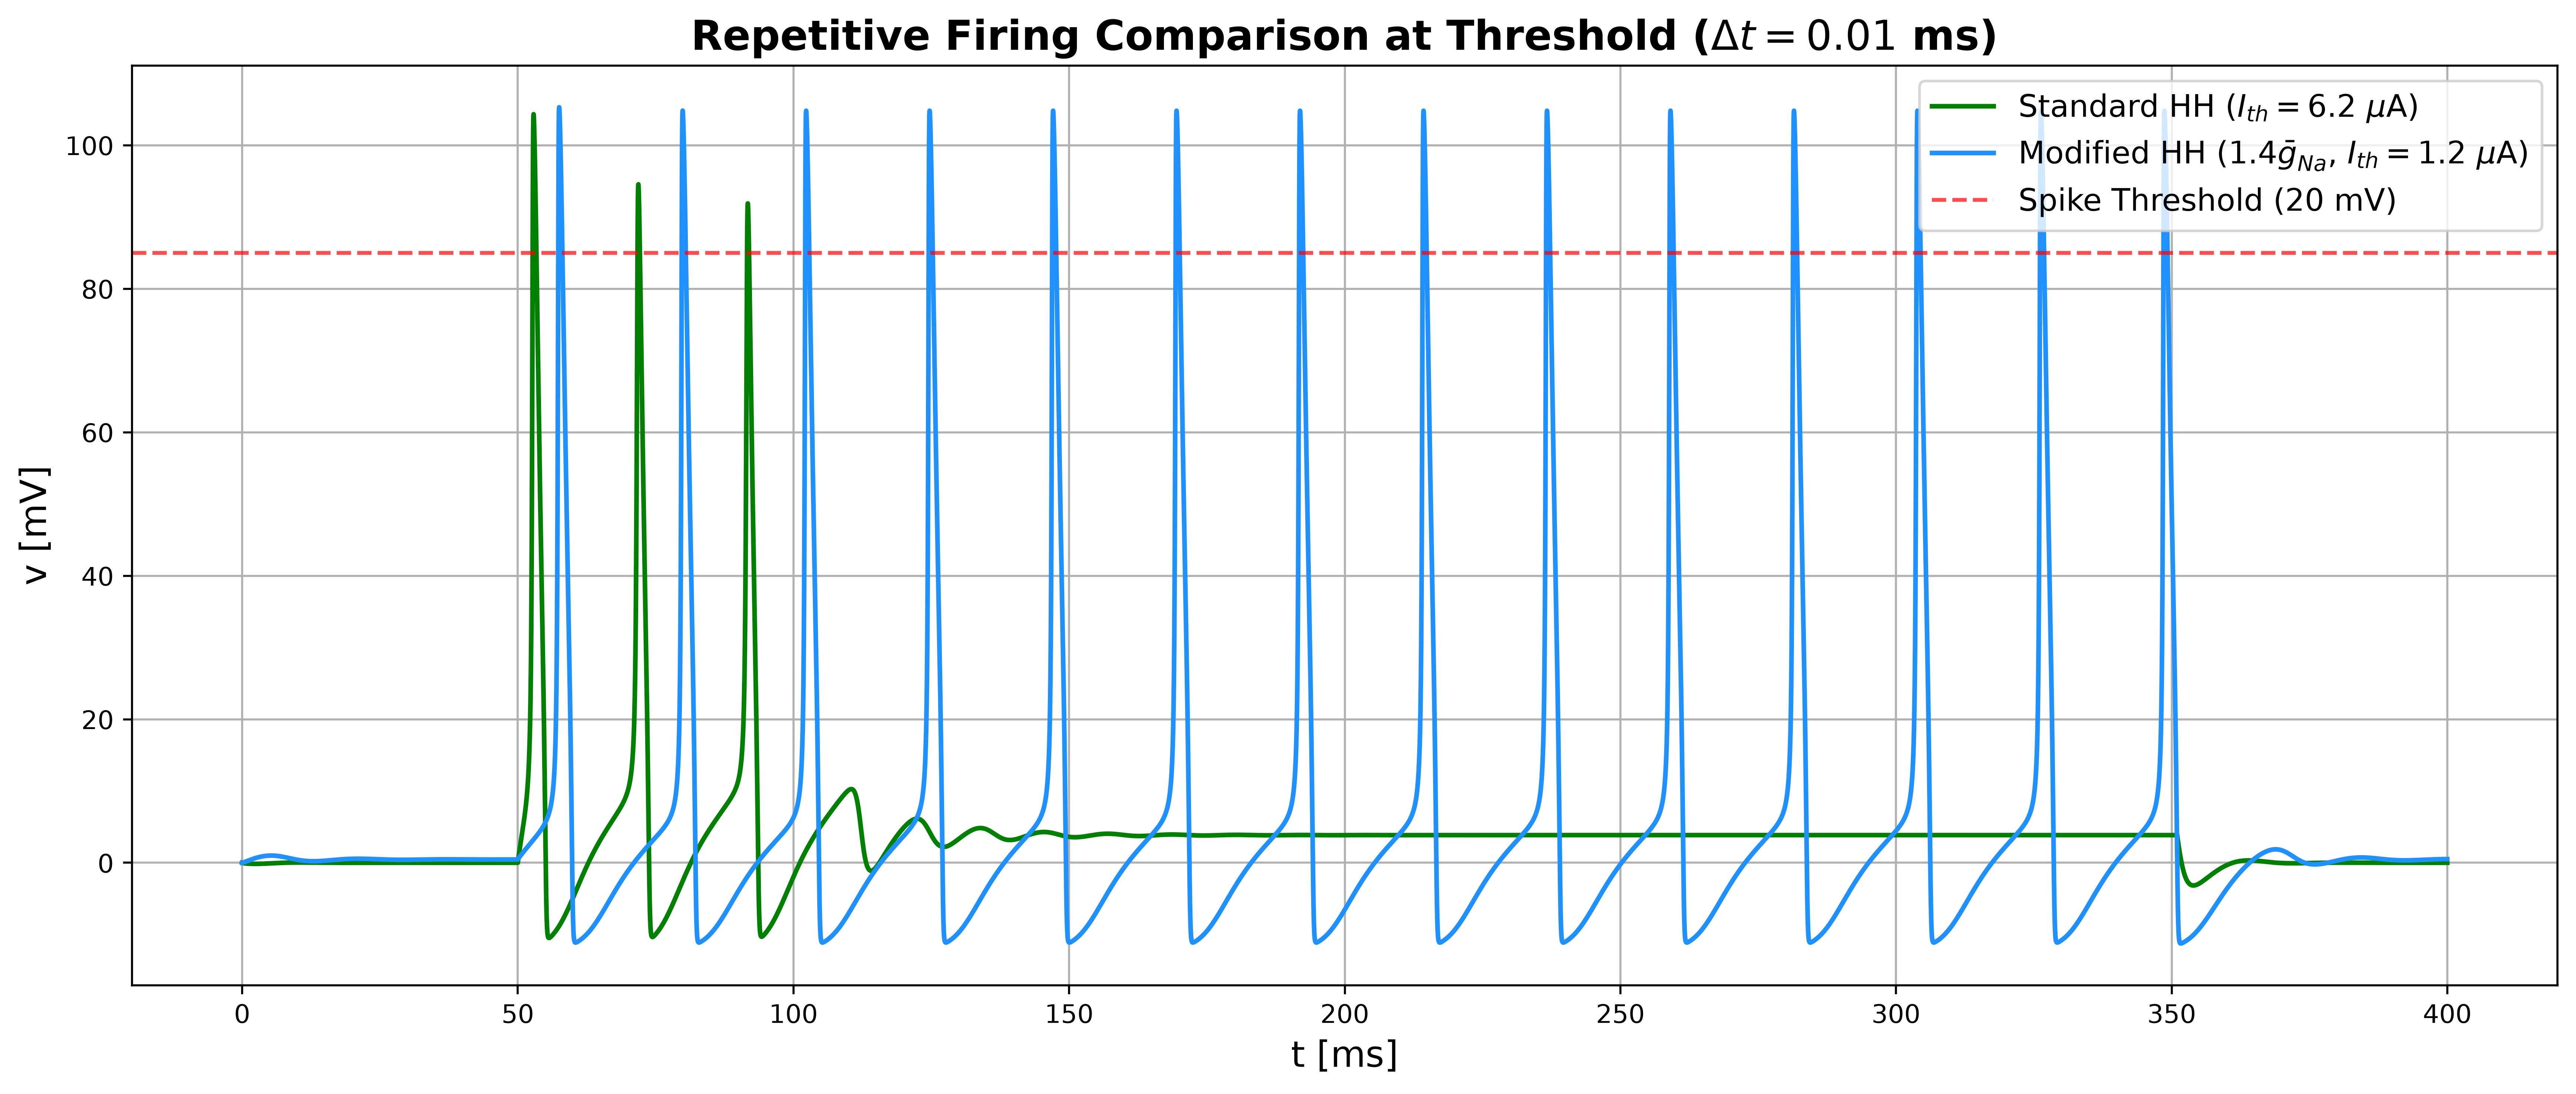
\includegraphics[width=0.94\textwidth]{../figures/q2/comparison_threshold_0.01.png}
\caption{Direct comparison of the two models at their respective measured repetitive-firing thresholds, using $\Delta t=0.01\,\mathrm{ms}$.}
\label{fig:q2comparison01}
\end{figure}
\begin{figure}[H]
\centering
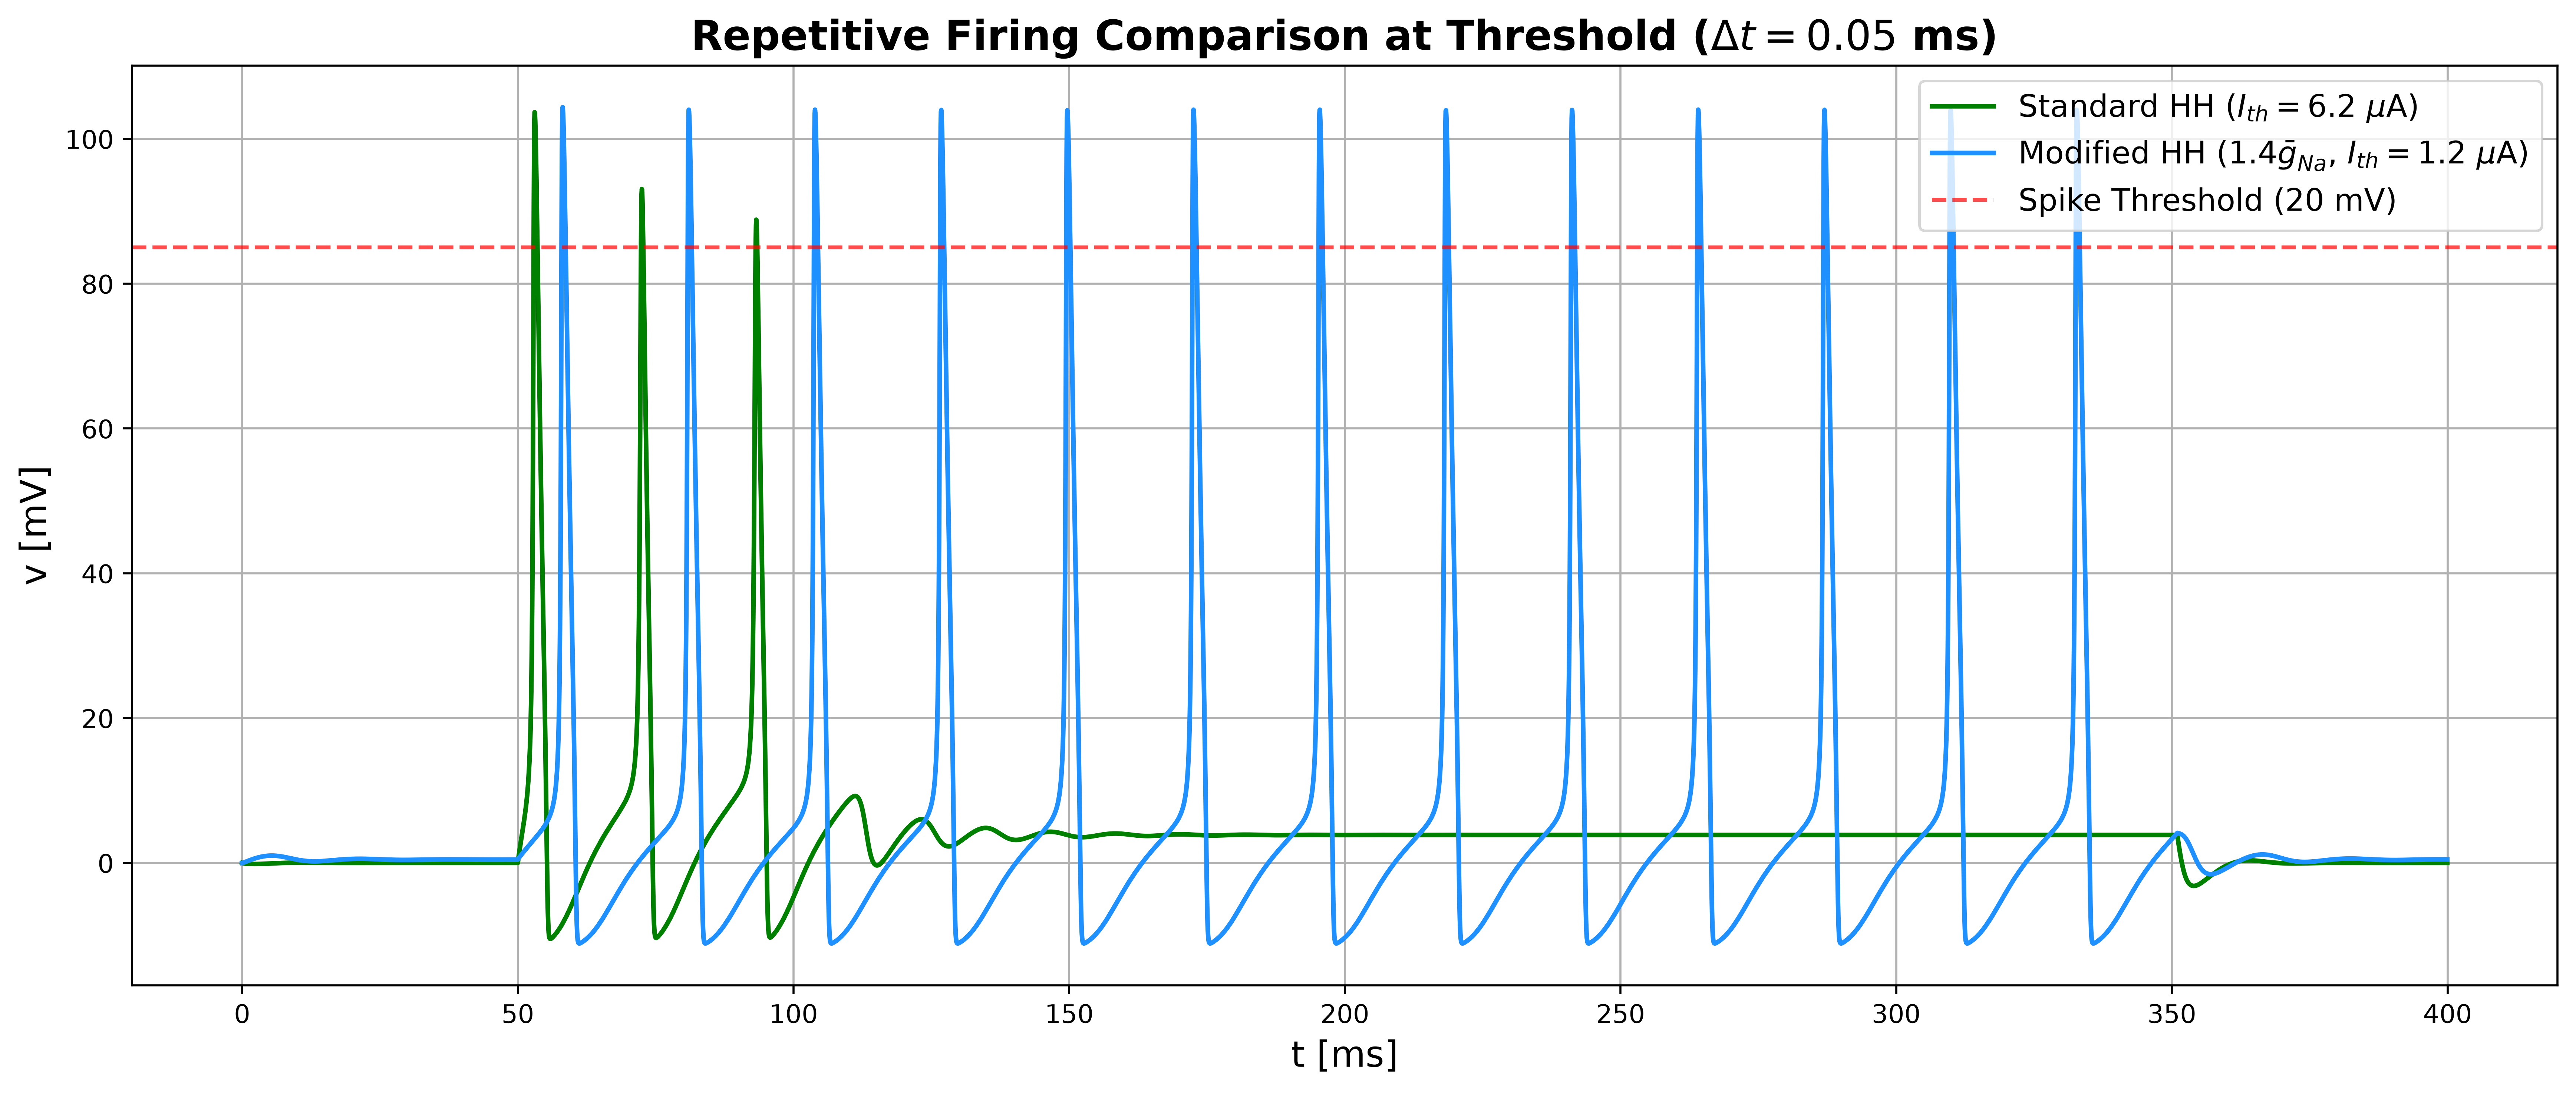
\includegraphics[width=0.94\textwidth]{../figures/q2/comparison_threshold_0.05.png}
\caption{The same threshold comparison at the coarser search timestep, $\Delta t=0.05\,\mathrm{ms}$.}
\label{fig:q2comparison05}
\end{figure}

\begin{figure}[H]
\centering
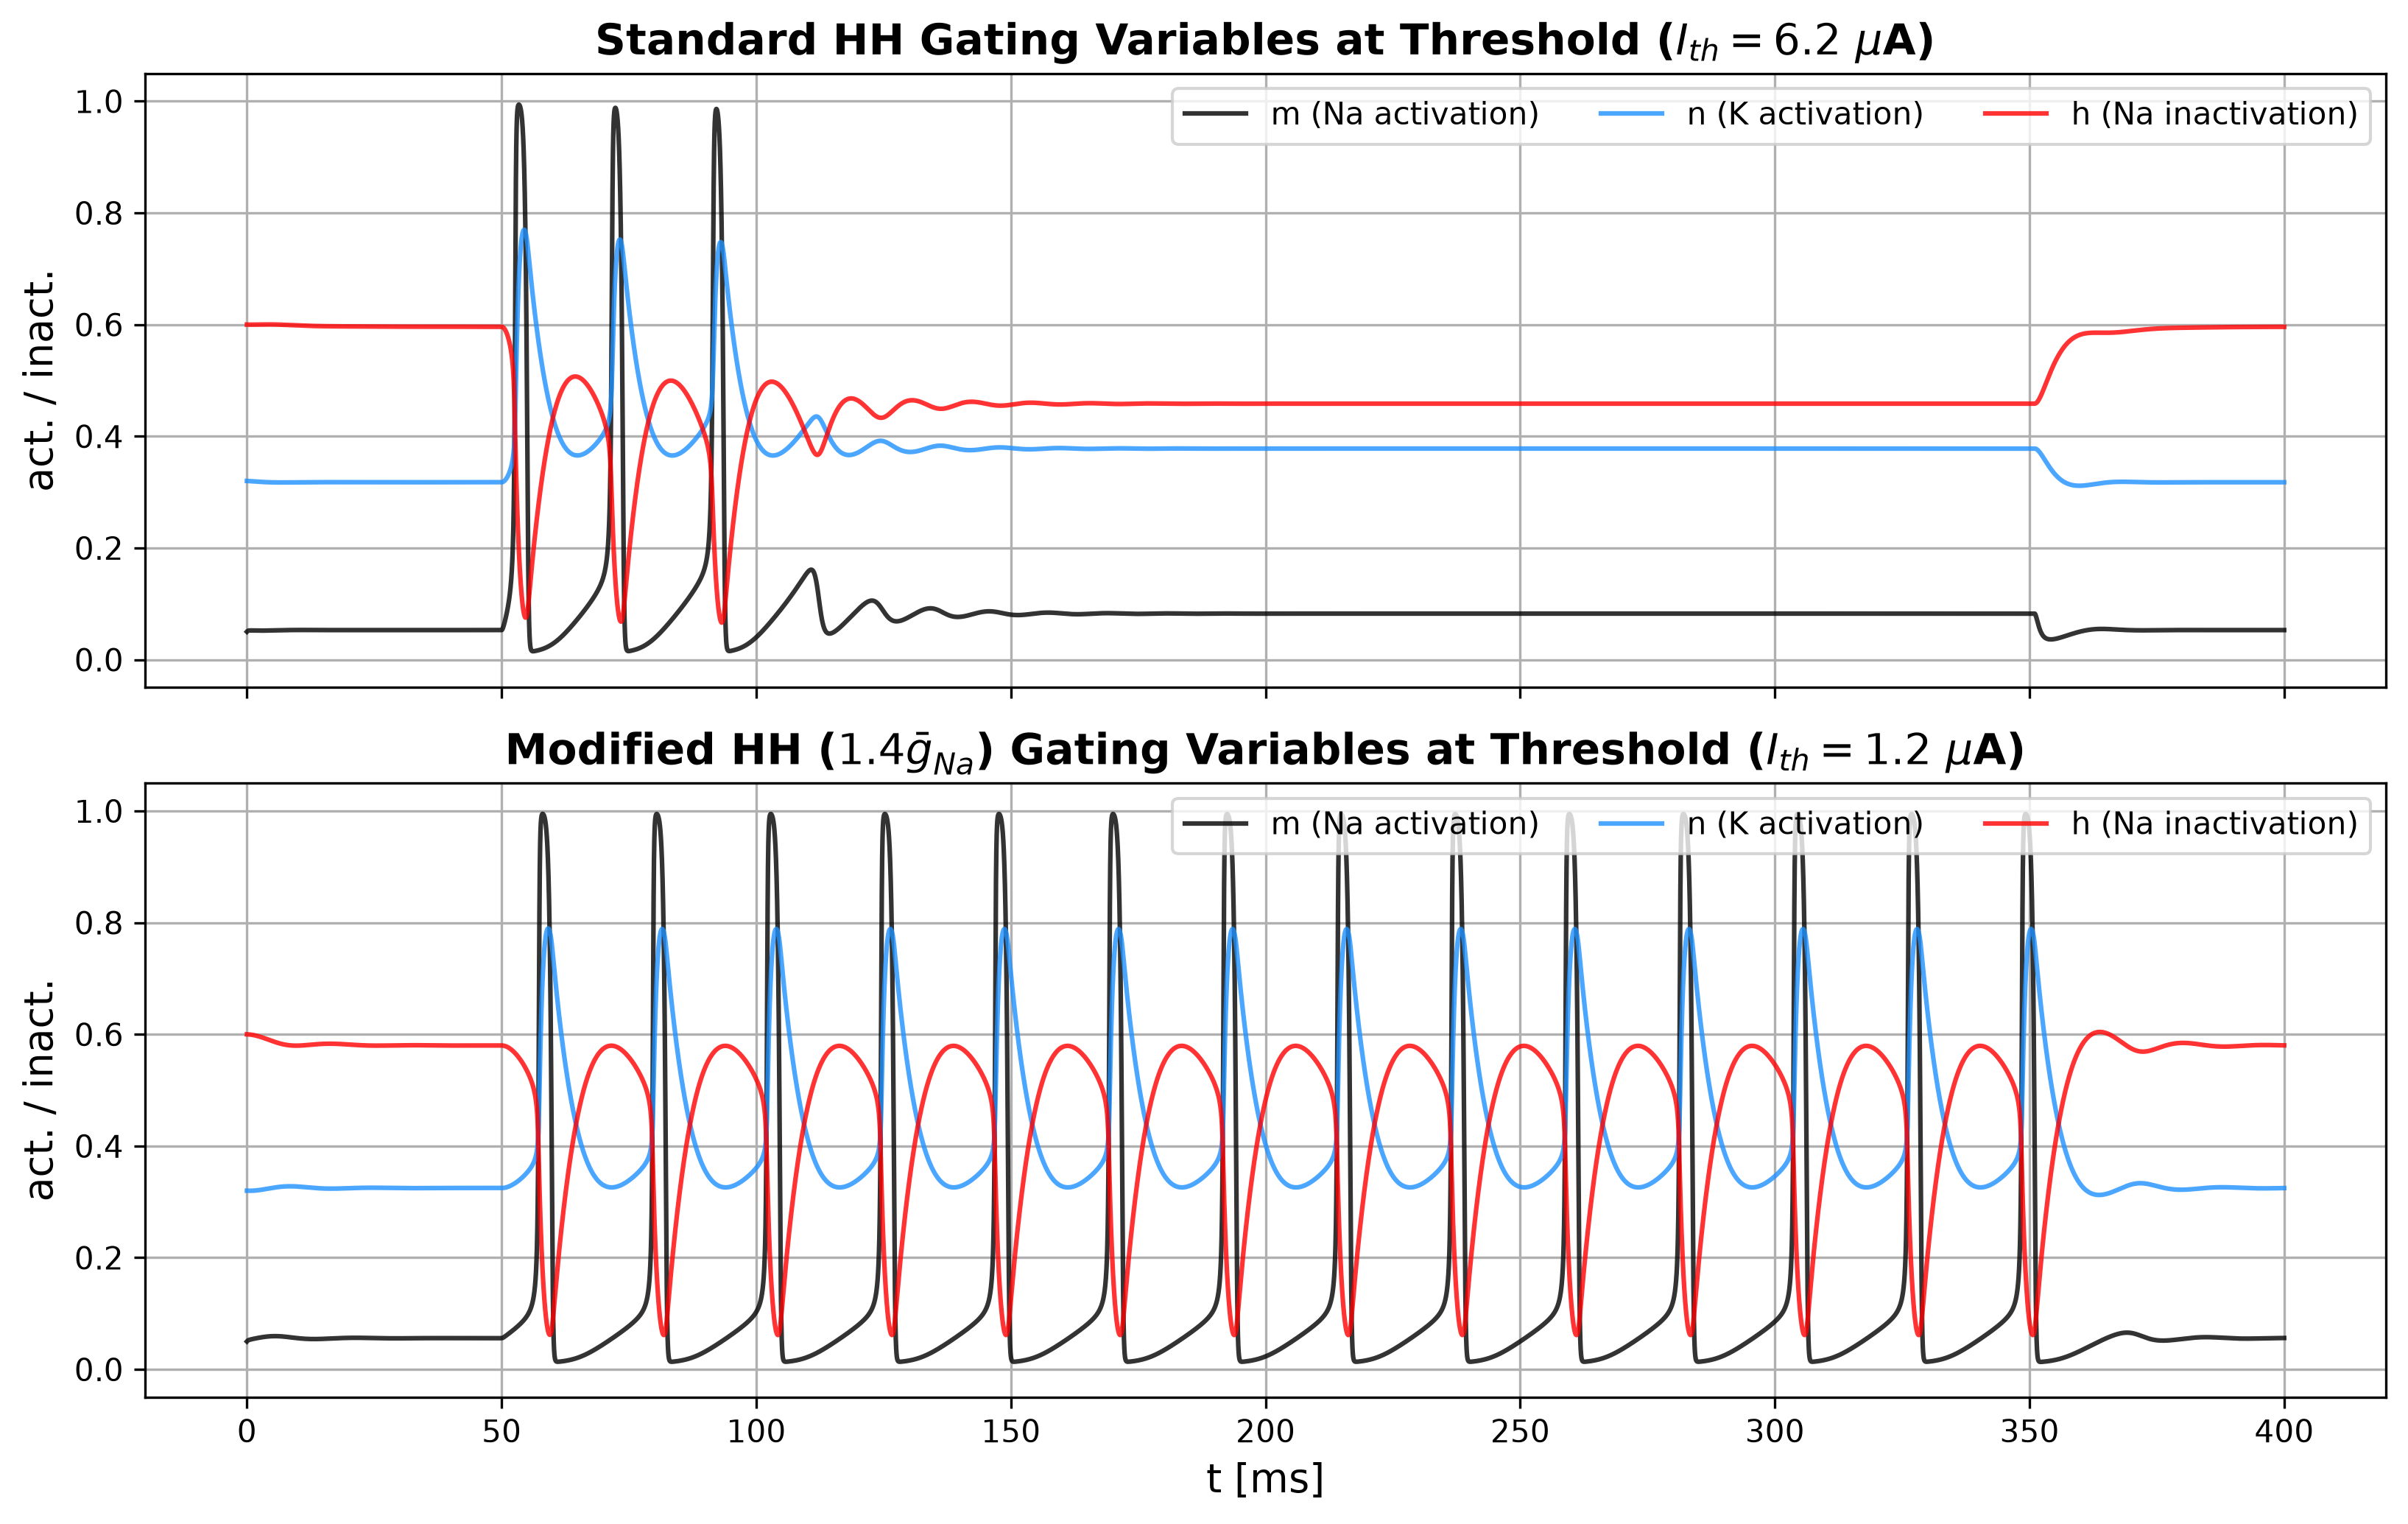
\includegraphics[width=0.94\textwidth]{../figures/q2/gating_comparison_threshold.png}
\caption{Standard and modified HH gating variables at their respective measured repetitive-firing thresholds.}
\label{fig:q2gating}
\end{figure}

Figures~\ref{fig:q2comparison01} and~\ref{fig:q2comparison05} show the same
model comparison at the two integration steps. The $0.01\,\mathrm{ms}$ plots are
the final high-resolution traces; the $0.05\,\mathrm{ms}$ plot documents the
resolution used during the threshold search. The table values are defined by the
search criterion, not by the visual height of the voltage traces.

\section*{Part B: Adding the Cav3.1 Calcium Channel}
\subsection*{Q3: Channel characterization and kinetics}
Cav3.1 is a low-threshold calcium channel with one activation gate
$m_{\mathrm{Ca}}$ and one inactivation gate $h_{\mathrm{Ca}}$, each with power one.
The Channelpedia reversal potential is $E_{\mathrm{Ca,CP}}=30\,\mathrm{mV}$. The HH
implementation uses $E_{\mathrm{Ca,HH}}=95\,\mathrm{mV}$ and
$V_{\mathrm{CP}}=V_{\mathrm{HH}}-65\,\mathrm{mV}$.

The implemented current is
\begin{equation}
 I_{\mathrm{Ca}}=\bar g_{\mathrm{Ca}}m_{\mathrm{Ca}}h_{\mathrm{Ca}}
 (E_{\mathrm{Ca}}-V),
\end{equation}
which is inward and depolarizing for $V<E_{\mathrm{Ca}}$. The gate dynamics are
\begin{align}
\frac{dm_{\mathrm{Ca}}}{dt}&=\frac{m_{\infty}(V)-m_{\mathrm{Ca}}}{\tau_m(V)},\\
\frac{dh_{\mathrm{Ca}}}{dt}&=\frac{h_{\infty}(V)-h_{\mathrm{Ca}}}{\tau_h(V)},\\
m_{\infty}(V)&=\frac{1}{1+\exp\left((V+42.921064)/(-5.163208)\right)},\\
h_{\infty}(V)&=\frac{1}{1+\exp\left((V+72.907420)/4.575763\right)},\\
\tau_m(V)&=\begin{cases}
-0.855809+1.493527\exp(-V/27.414182)\,\mathrm{ms},&V<-10\,\mathrm{mV},\\
1.0\,\mathrm{ms},&V\geq-10\,\mathrm{mV},
\end{cases}\\
\tau_h(V)&=9.987873+0.002883\exp(-V/5.598574)\,\mathrm{ms}.
\end{align}

\begin{figure}[H]
\centering
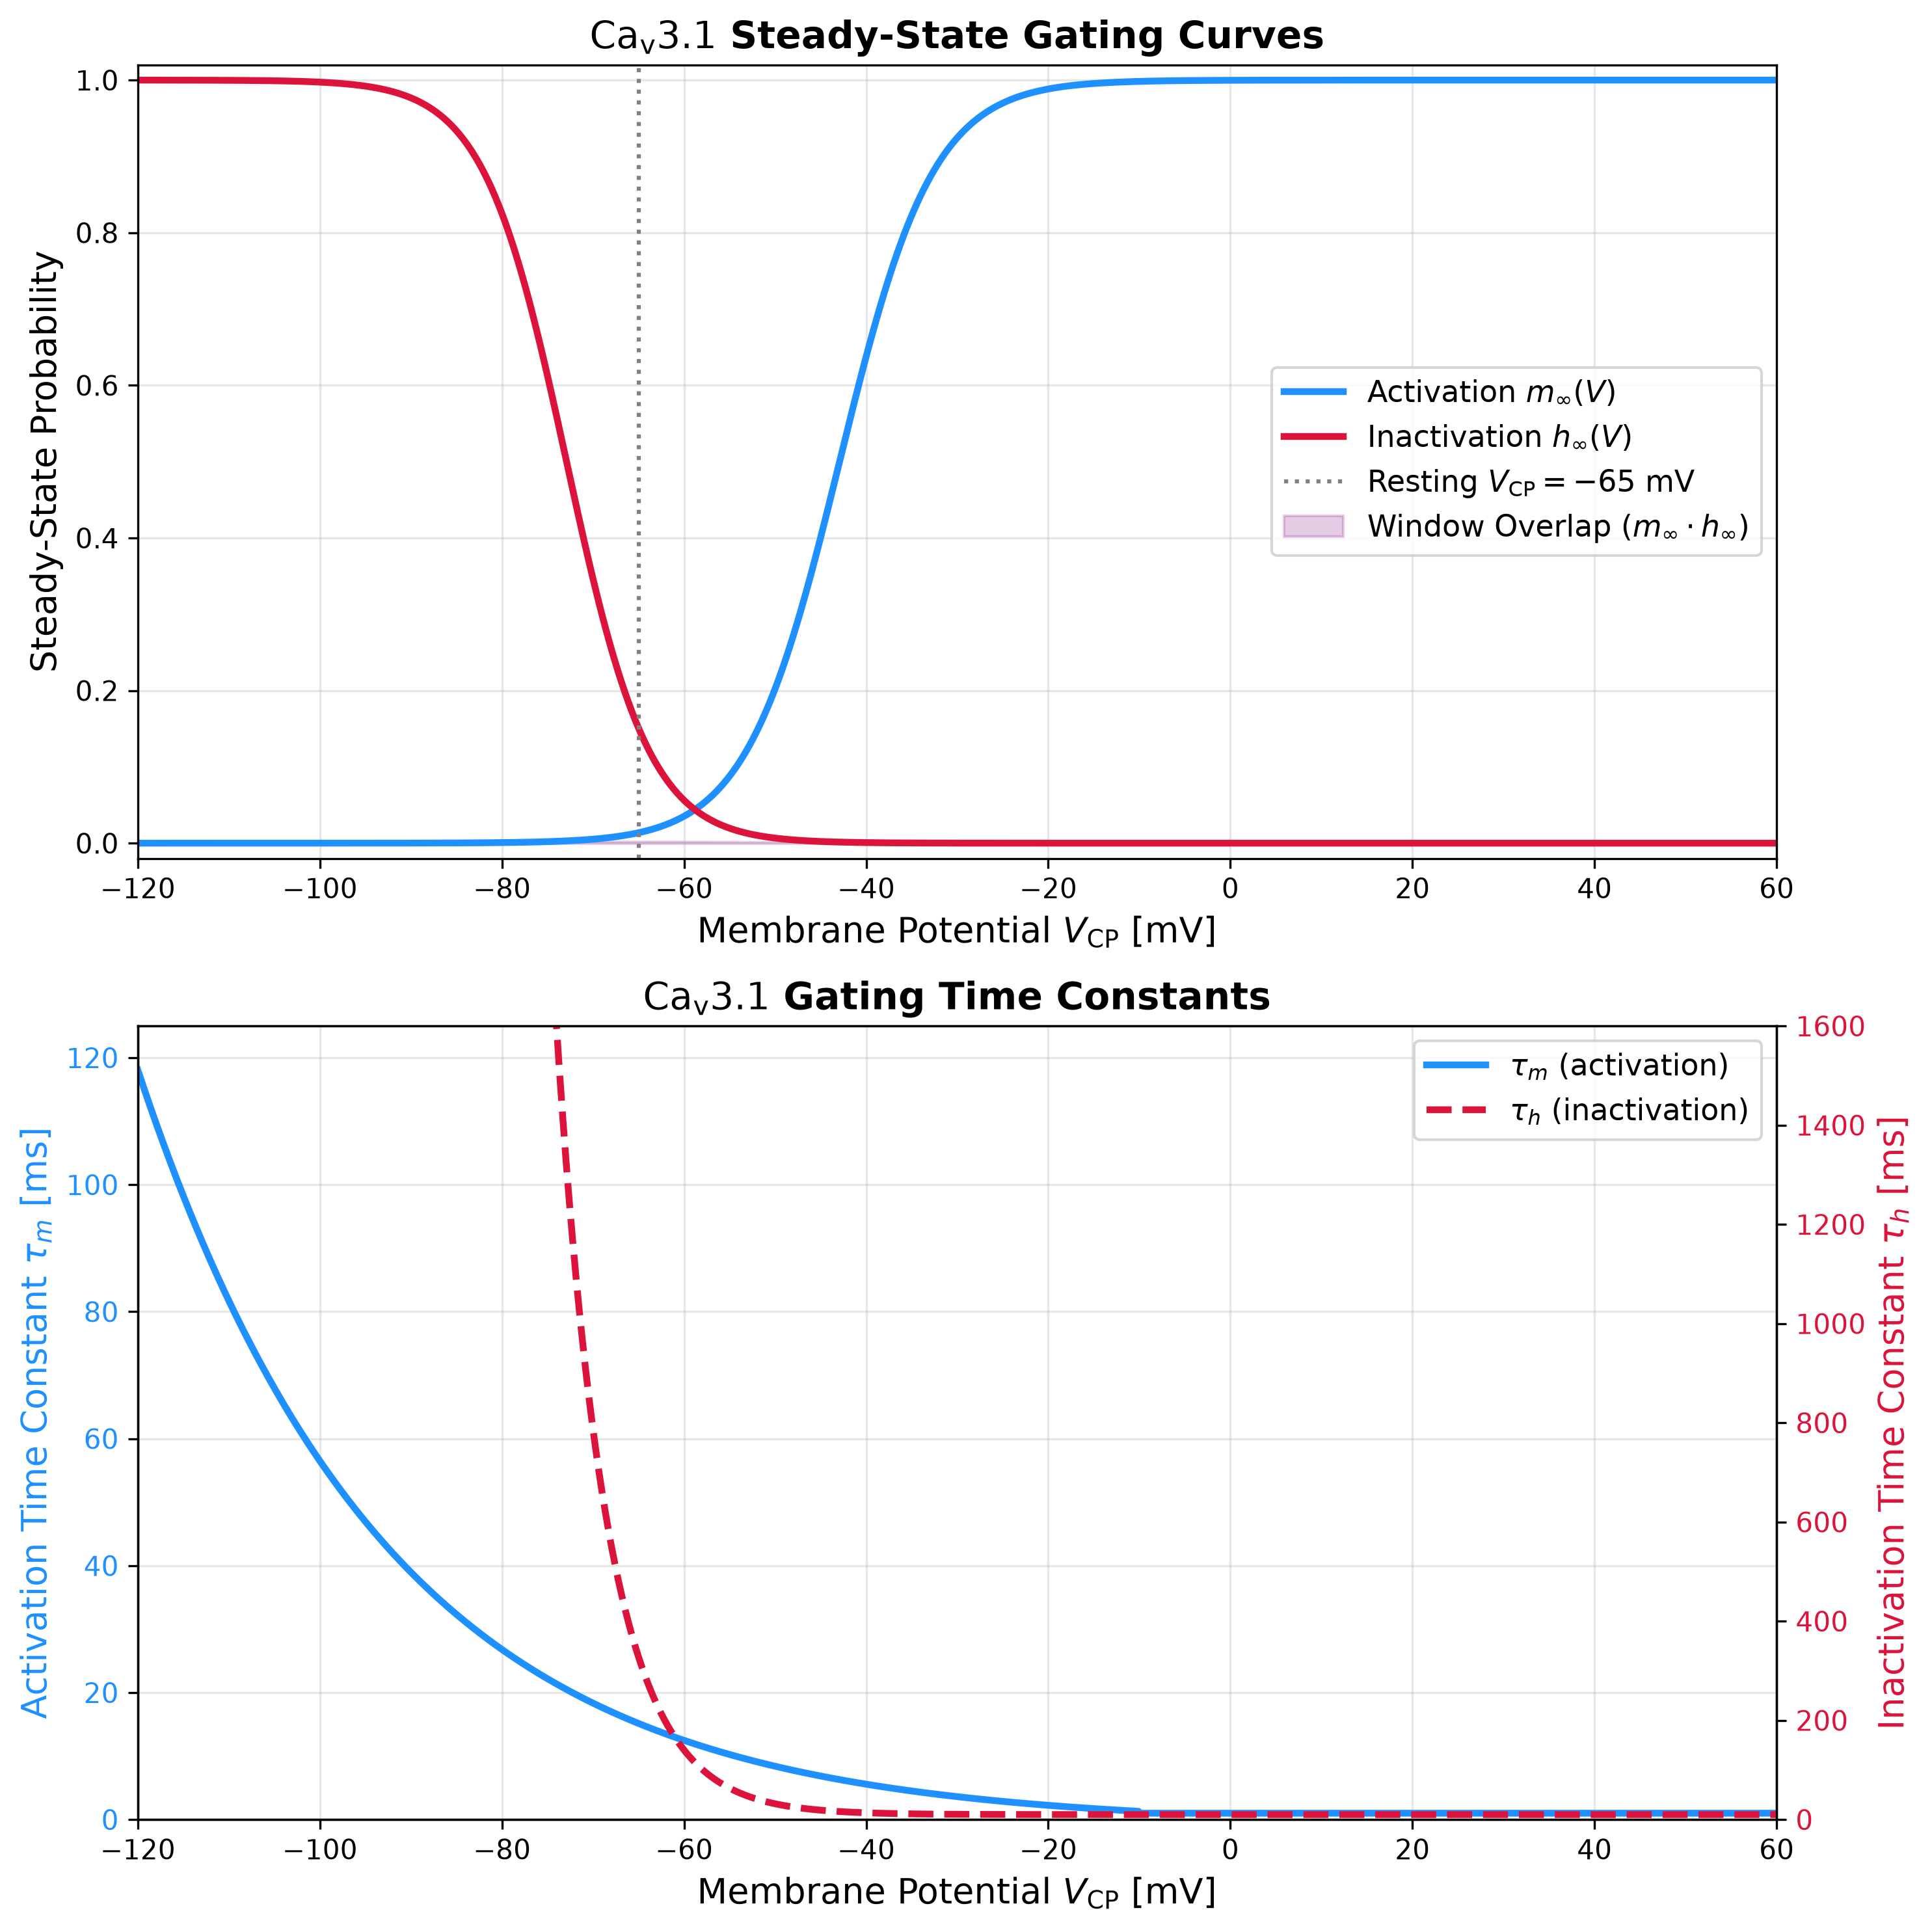
\includegraphics[width=0.88\textwidth]{../figures/q3/cav3_1_kinetics_stacked.png}
\caption{Cav3.1 steady-state gating variables and voltage-dependent time constants.}
\label{fig:q3}
\end{figure}

At hyperpolarized voltages, $h_{\infty}$ is large but $m_{\infty}$ is small: the
channel is available but mostly closed. During depolarization, $m_{\infty}$ rises
while $h_{\infty}$ falls. Thus, hyperpolarization primes a transient current by
removing inactivation, and release allows activation before inactivation has fully
recovered. The channel is therefore most relevant during a transient excursion
through approximately $-55$ to $-35\,\mathrm{mV}$ in Channelpedia coordinates,
where activation has begun but inactivation has not yet eliminated availability.
The activation gate is faster than the inactivation gate, so a brief overlap of
$m_{\mathrm{Ca}}$ and $h_{\mathrm{Ca}}$ is possible after hyperpolarization.

\subsection*{Q4: Rebound response after hyperpolarization}
The extended model uses $\bar g_{\mathrm{Ca}}=20\,\mathrm{mS}$ and applies a
$-2.0\,\mu\mathrm{A}$ step from $50$ to $250\,\mathrm{ms}$. Both models are
simulated for $350\,\mathrm{ms}$ with $\Delta t=0.01\,\mathrm{ms}$.

\begin{figure}[H]
\centering
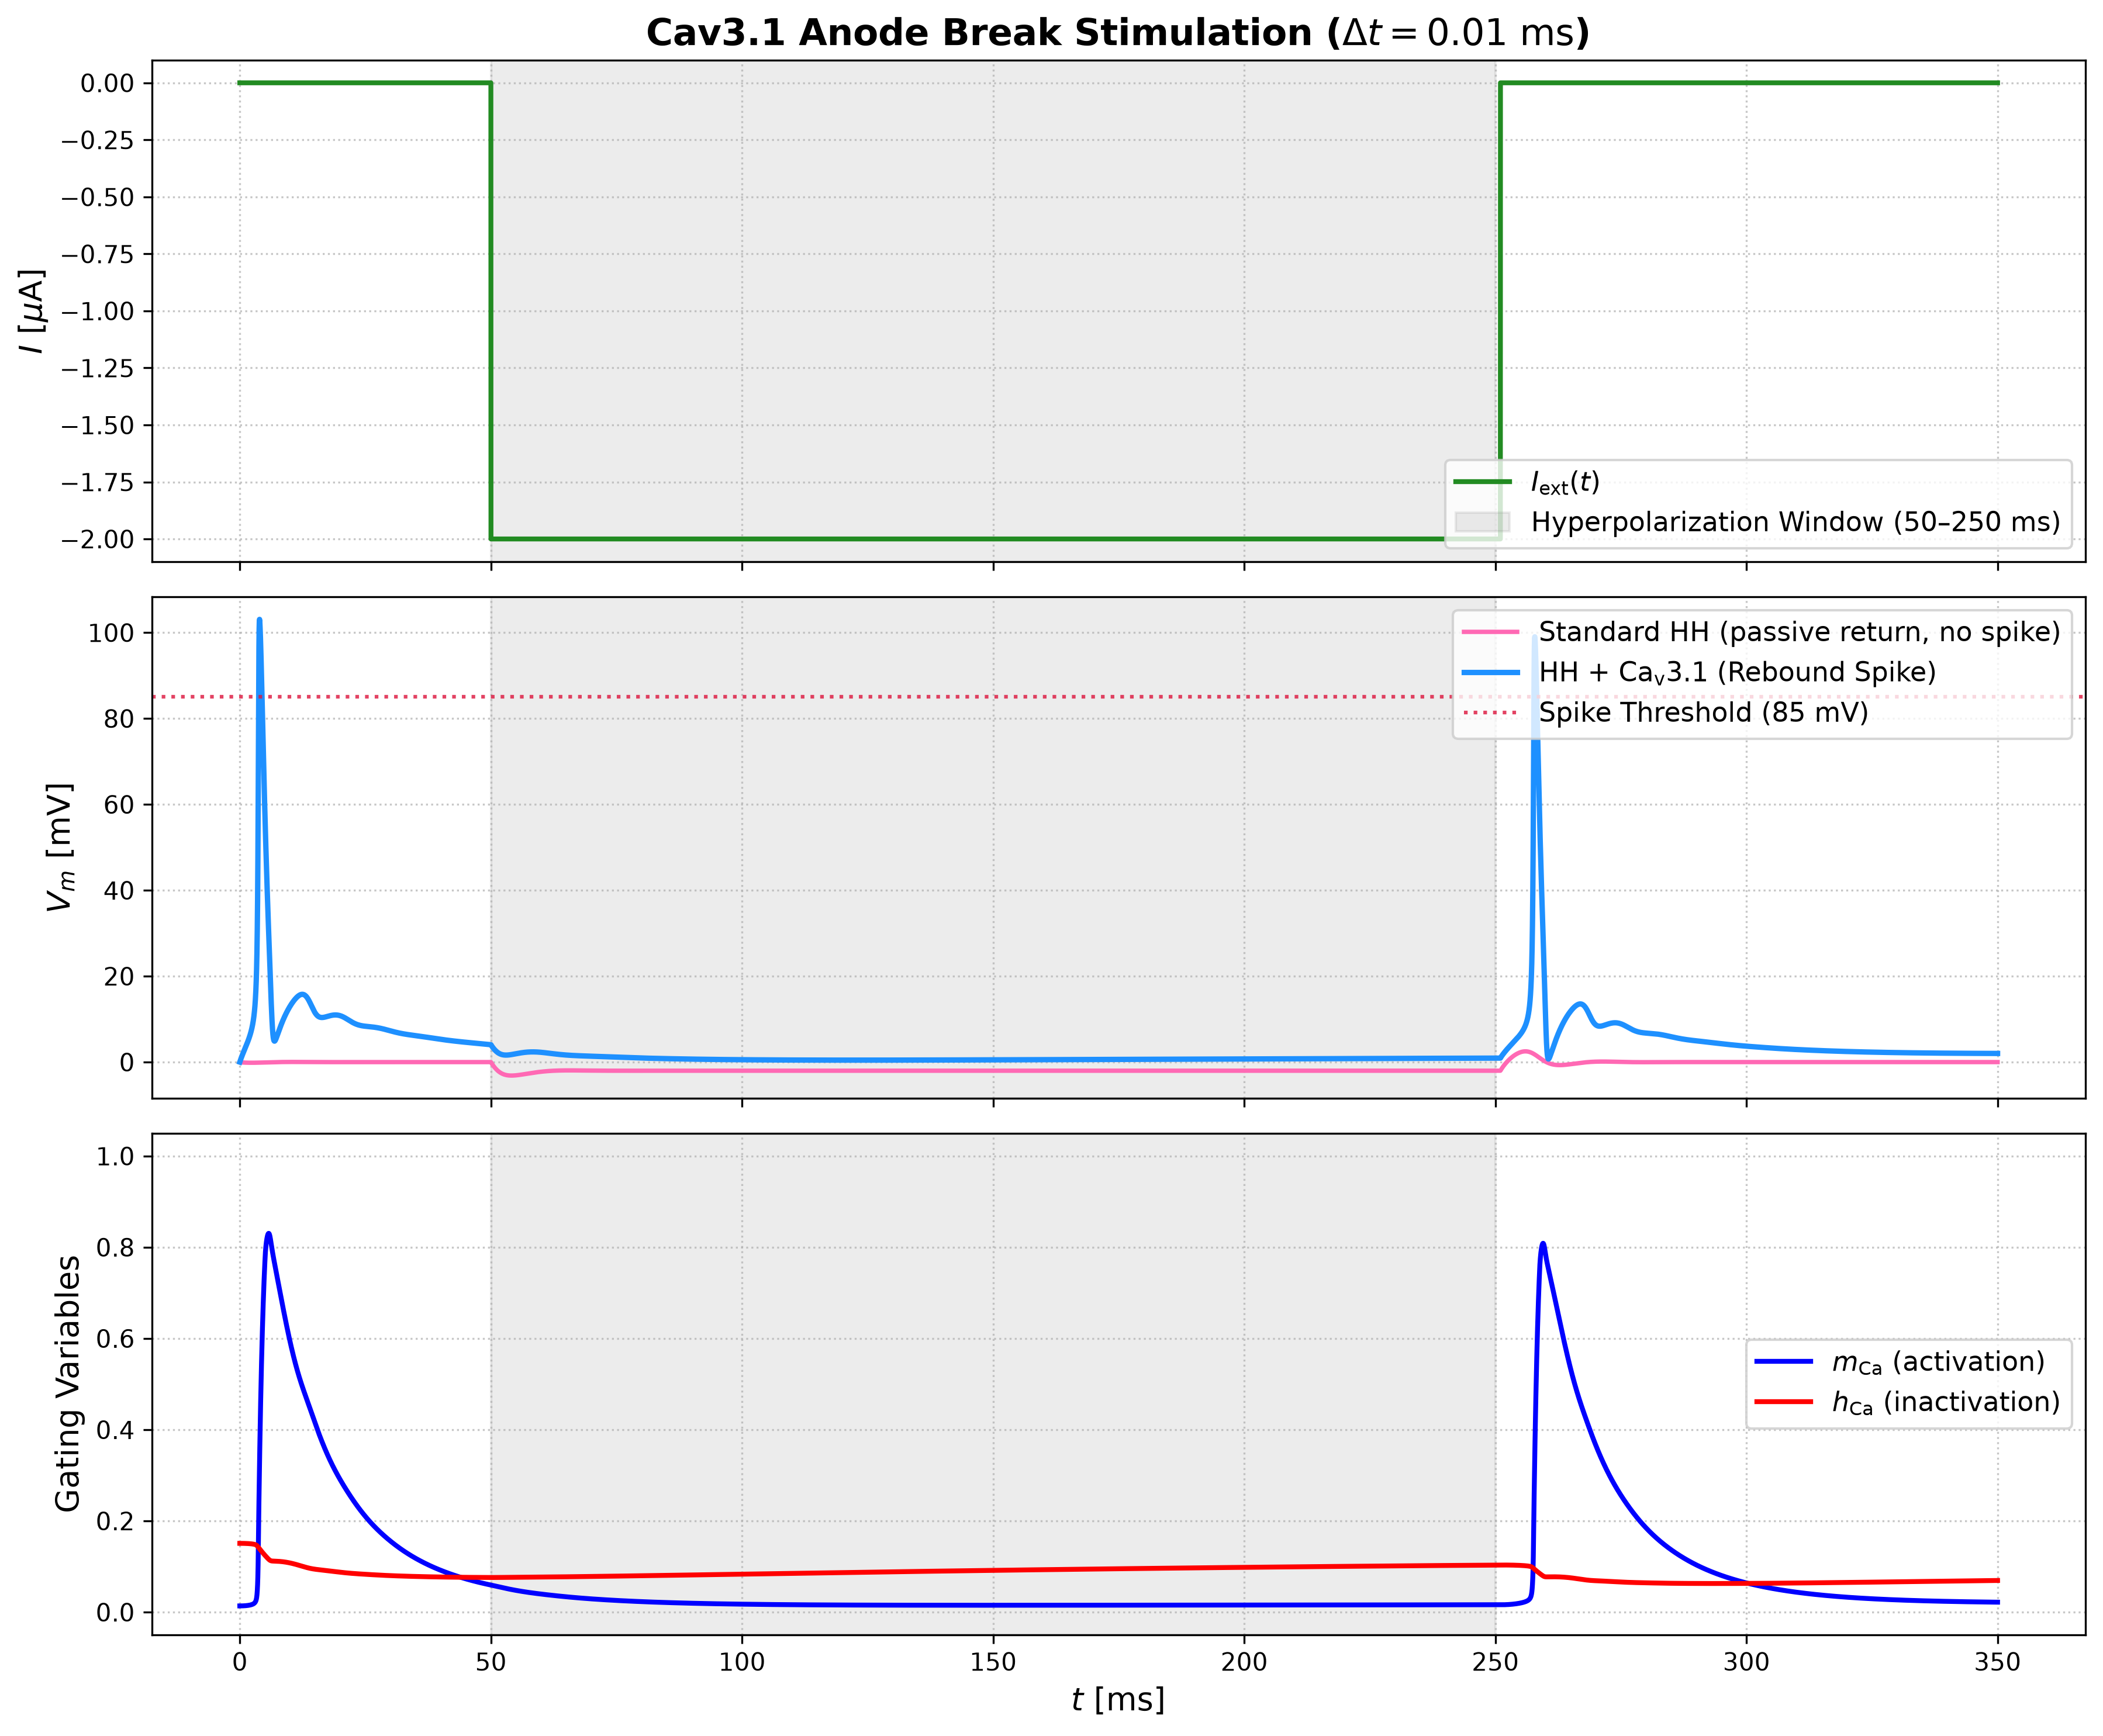
\includegraphics[width=0.97\textwidth]{../figures/q4/cav31_rebound_simulation.png}
\caption{Anode-break stimulation: hyperpolarization primes Cav3.1, followed by a rebound spike after current removal.}
\label{fig:q4}
\end{figure}

During the negative-current interval, $h_{\mathrm{Ca}}$ increases while
$m_{\mathrm{Ca}}$ remains small. When the current is removed at $250\,\mathrm{ms}$,
the membrane returns toward rest. Activation of $m_{\mathrm{Ca}}$ overlaps with the
still-large $h_{\mathrm{Ca}}$, producing an inward calcium current that depolarizes
the membrane enough to recruit the standard sodium current. The standard HH comparison
returns toward rest without the corresponding rebound event.

For the saved notebook run, the rebound peak is $99.02\,\mathrm{mV}$ at
$257.84\,\mathrm{ms}$, giving a peak latency of $7.84\,\mathrm{ms}$. The first
crossing of the analysis threshold $20\,\mathrm{mV}$ occurs at $257.68\,\mathrm{ms}$,
giving a threshold-crossing latency of $7.68\,\mathrm{ms}$.

\section*{Conclusion}
The simulations demonstrate two mechanisms of excitability. In the classical HH
model, sodium conductance controls regenerative positive feedback and strongly changes
the current required for repetitive firing. In the extended model, Cav3.1 provides a
memory of prior hyperpolarization: its inactivation gate is relieved during the
negative-current pulse, and release produces a transient inward calcium current. The
rebound spike is therefore a direct consequence of voltage-dependent activation and
inactivation kinetics.

\end{document}
